\documentclass[12pt]{article}
\usepackage[spanish]{babel}
\usepackage{graphicx}

\title{Síntesis de redes activas laboratorio Nº1: Amplificadores ideales lineales y no lineales}

\author{Profesor Titular: Dr. Ing. Pablo Ferreyra \\  Profesor Adjunto: Ing. César Reale \\ Alumnos: Campos Mariano, 
		Enzo Verstraete}

\begin{document}
	\maketitle
	
	\begin{abstract}
		Primer laboratorio cuyo objetivo es familiarizarse con el armado y análisis de circuitos analógicos
		lineales y no lineales. En este Trabajo Práctico debe considerar para los cálculos iniciales el
		amplificador como ideal. \newpage
	\end{abstract}
	
	
	\section{Metodología general}	
		A. Realizar una sintética introducción teórica del tema a tratar.
		B. Analizar los circuitos propuestos, todos los cálculos analíticos y su desarrollo numérico.
		C. Simulación en SPICE .
		D. Analizar las condiciones de operación límite.
		E. Armar el circuito y hacer las mediciones en laboratorio.
		F. Finalmente comparar los valores calculados, simulados y medidos, y extraer conclusiones a
		cerca de las diferencias. Analizar las causas.
		G. Presentar un informe digital, bien redactado en LÁTEX, inicializado con la propuesta del
		problema presentado por la Cátedra, los responsables del trabajo y un análisis profesional de
		cada ítem. La redacción debe ser acorde a un informe de un futuro ingeniero.
		
	\section{Circuito I: Amplificador diferencial}
		\subsection{Introducción al análisis}
		
		El análisis del	circuito tiene como objetivo obtener una primera aproximación del comportamiento
		del circuito de manera rápida y eficiente. Para dicho análisis se tienen en cuenta las siguientes
		consideraciones.
		
		Ganancia infinita: Al considerar una ganancia infinita, la diferencia de tensión entre las entradas inversora y no inversora se hace prácticamente cero. Esto permite aplicar el concepto de "masa virtual" en la entrada inversora, simplificando notablemente el análisis.
		
		Impedancia de entrada infinita: La alta impedancia de entrada implica que prácticamente no circula corriente hacia las entradas del operacional, lo que facilita la aplicación de la Ley de Kirchhoff de las Corrientes (KCL) en los nodos de entrada.
		
		Impedancia de salida nula: Al considerar una impedancia de salida nula, se asume que el operacional puede suministrar cualquier cantidad de corriente sin que su tensión de salida se vea afectada, lo que simplifica el análisis de la carga conectada a la salida.
		
		En esta sección se analiza el siguiente circuito.
		\begin{figure}
			\centering
			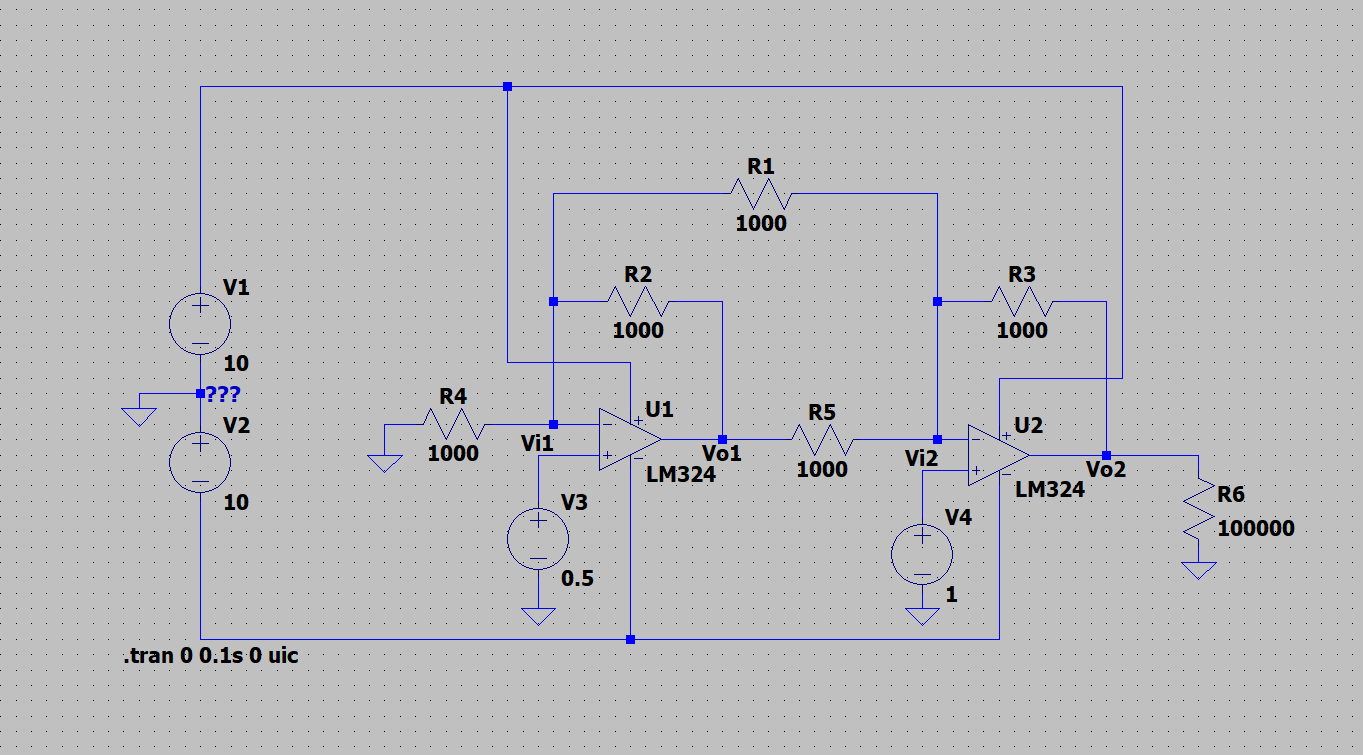
\includegraphics[width=1\linewidth]{Simulaciones-Resultados/Circuito1_esquematico}
			\caption{Amplificador diferencial}
			\label{fig:circuito1esquematico}
		\end{figure} \newpage
		
		\subsection{Análisis del circuito}
		Para el análisis podemos hacer uso de la propiedad de superposición, considerando la salida como la suma de los
		efectos individuales de las distintas excitaciones del circuito:
		
		Análisis de $V_{01}$ por superposición de $V_1$ y $V_2$:
		
		Para $V_2=0$ queda un amplificador no inversor de $R_2$ sobre el paralelo $R_1$ y $R_4$
		\begin{equation}
			V_{01} = V_1 \,{\left(\frac{R_2 \,{\left(R_1 +R_4 \right)}}{R_1 \,R_4 }+1\right)}
		\end{equation}
		
		Normalizando los valores de la resistencia obtenemos:
		\begin{equation}
			R_1=R_2=R_3=R 
		\end{equation}
		
		La salida de $V01$ resulta:
		\begin{equation}
			V_{01}=3\,V_1
		\end{equation}
		
		Para $V_1=0$ tenemos que
		\begin{equation}
			V_{01} = -\frac{R_2 \,V_2 }{R_5 }
		\end{equation}
		
		Normalizando los valores de la resistencia obtenemos:
		\begin{equation}
			R_2=R_5=R 
		\end{equation}
		
		La salida de $V01$ resulta:
		\begin{equation}
			V_{01}=-V_2
		\end{equation}
		
		La salida de $V_{01}$ resulta la suma de ambos efectos, se obtiene:
		\begin{equation}
			V_{01}=3\,V_1-V_2
		\end{equation}
		
		Análisis de $V_{02}$ por superposición de $V_1$, $V_2$ y $V_{01}$:
		
		Para $V_1=0$ y $V_2=0$  tenemos una configuración inversora de $R_3$ sobre $R_5$
		\begin{equation}
			V_{02}=-\frac{R_3 \,V_{01} }{R_5 }
		\end{equation}
		
		Normalizando los valores de la resistencia obtenemos:
		\begin{equation}
			R_3=R_5=R 
		\end{equation}
		
		La salida de $V_{01}$ resulta:
		\begin{equation}
			V_{02}=-V_{01}
		\end{equation}
		
		Para $V_1=0$ y $V_{01}=0$ queda un amplificador no inversor de $R_3$ sobre el paralelo $R_1$ y $R_5$
		\begin{equation}
			V_{02} = V_2 \,{\left(\frac{R_3 \,{\left(R_1 +R_5 \right)}}{R_1 \,R_5 }+1\right)}
		\end{equation}
		
		Normalizando los valores de la resistencia obtenemos:
		\begin{equation}
			R_1=R_3=R_5=R 
		\end{equation}
		
		La salida de $V_{02}$ resulta:
		\begin{equation}
			V_{02}=3\,V_2
		\end{equation}
		
		Para $V_2=0$ y $V_{01}=0$  tenemos una configuración inversora de $R_3$ sobre $R_4$
		\begin{equation}
			V_{02}=-\frac{R_3 \,V_1 }{R_4 }
		\end{equation}
		
		Normalizando los valores de la resistencia obtenemos:
		\begin{equation}
			R_3=R_4=R 
		\end{equation}
		
		La salida de $V_{02}$ resulta:
		\begin{equation}
			V_{02}=-V_1
		\end{equation}
		
		La salida de $V_{02}$ resulta la suma de los tres efectos, se obtiene:
		\begin{equation}
			V_{02}=3\,V_2-V_1-V_{01}
		\end{equation}
		
		Reemplazando (7) en la ecuación anterior, se obtiene la respuesta total del circuito
		\begin{equation}
			V_{02}=4\,(V_2-V_1)
		\end{equation}
		
		\subsection{Simulación en SPICE}
		
		\begin{figure}[h]
			\centering
			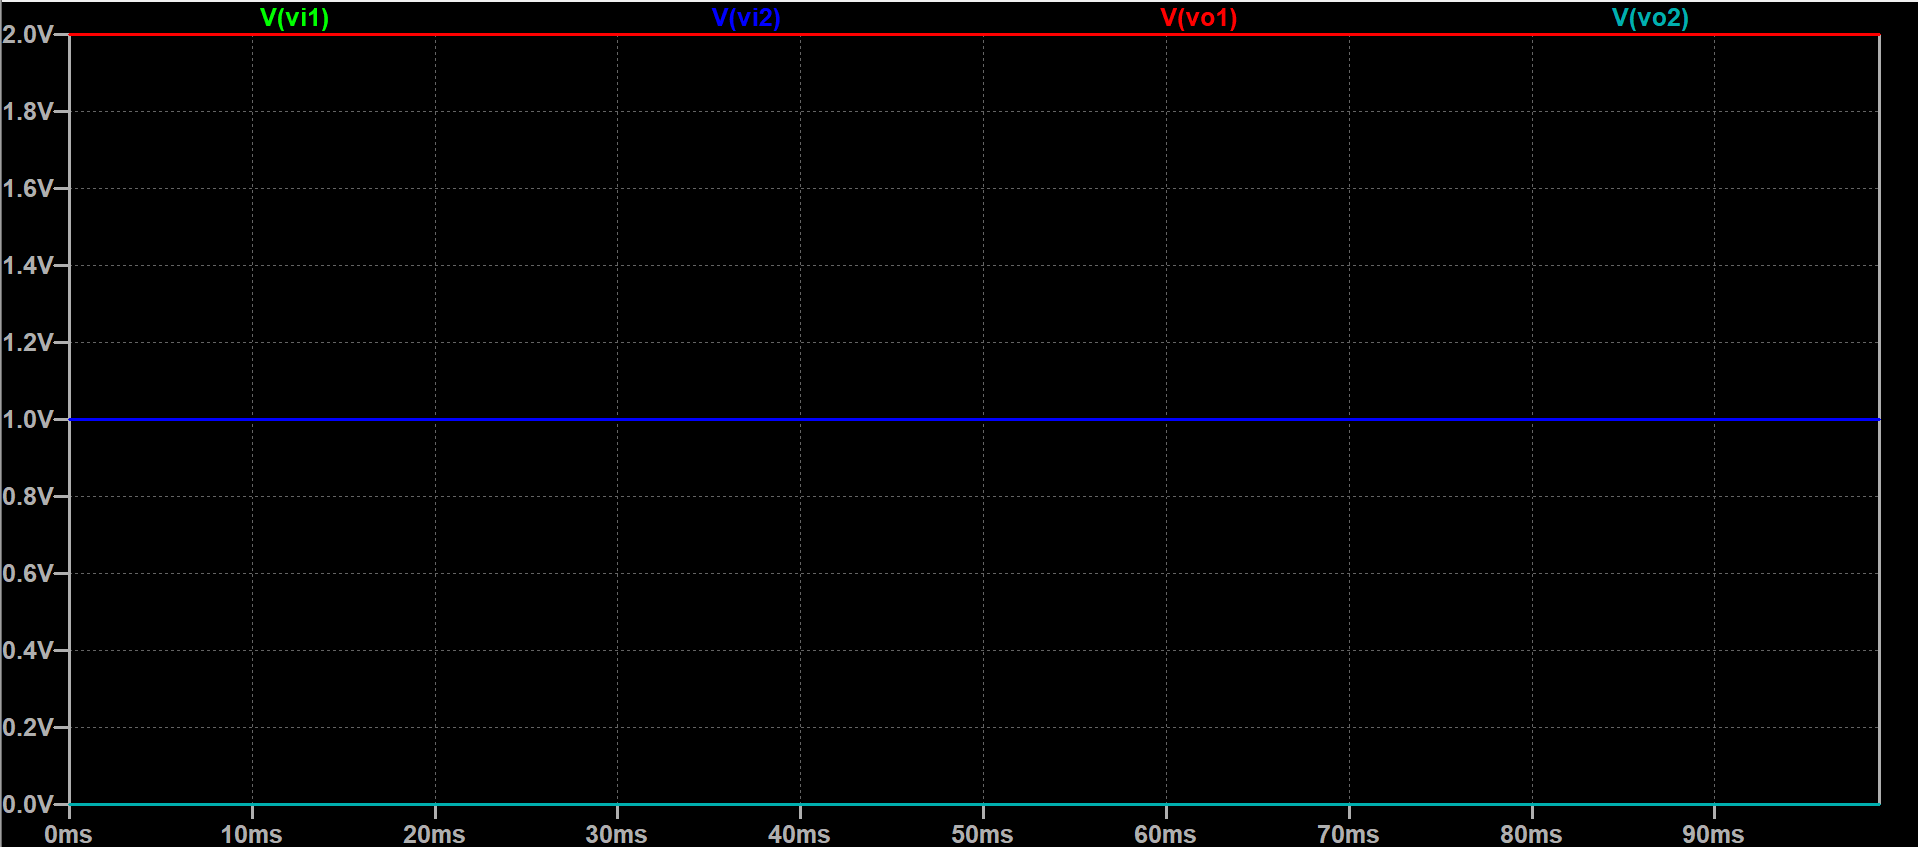
\includegraphics[width=1\linewidth]{Simulaciones-Resultados/Circuito1_Vo1(Vc)-Vo2(Vc)}
			\caption{Tensión en modo común}
			\label{fig:circuito1vo1vc-vo2vc}
		\end{figure} \newpage
		
		
		
		
		
		
		
		
\end{document}
	}